\documentclass[11pt,spanish]{article}

% =========================================================
% CONFIGURACIÓN GENERAL
% =========================================================

\usepackage[utf8]{inputenc}
\usepackage[T1]{fontenc}
\usepackage[spanish,es-lcroman,es-tabla]{babel}
\usepackage{graphicx}
\usepackage{booktabs}
\usepackage{array}
\usepackage{tabularx}
\usepackage{enumitem}
\usepackage{float}
\usepackage{pgfgantt}
\usepackage{caption}
\usepackage{comment}
\usepackage{url}
\usepackage{hyperref}
\usepackage[letterpaper,margin=2.2cm]{geometry}

% =========================================================
% DATOS DEL DOCUMENTO
% =========================================================

\title{Plataforma distribuida de comunicación y alertas comunitarias para entornos universitarios (Noti Uam)}
\author{Aaron Rodrigo Ramos Reyes}
\date{2026}


% =========================================================
% DOCUMENTO
% =========================================================
\begin{document}

% =========================================================
% PORTADA PERSONALIZADA (con Asesor)
% =========================================================

\begin{titlepage}
    \centering

    \vskip 1.5cm

    % Logo UAM
    
\includegraphics[width=0.8\textwidth]{imagenes/logo_uam.png}
    \vskip 1.5cm

    {\Large División de Ciencias de la Comunicación y Diseño}
    \vskip 0.2cm
    {\Large  Departamento de Tecnologías de la Información} 
    \vskip 0.2cm
    {\Large Licenciatura en Tecnologías y Sistemas de Información\par}
    \vskip 3cm

    {\Large\bfseries Protocolo de Proyecto Terminal I \par}
    \vskip 0.5cm

    {\Large \bfseries Plataforma distribuida de comunicación y alertas comunitarias para entornos universitarios: NotiUam\par}
    \vskip 2cm

    \begin{tabular}{rl}
        \textbf{Alumno:} & Aaron Rodrigo Ramos Reyes \\
        \textbf{Carrera:} & Sistemas y Tecnologías de Información \\
        \textbf{Trimestre:} & 26-P \\
        \textbf{Asesores:}   & Mtra. Betzabet García Mendoza\\      % <--- CAMBIAR POR EL NOMBRE REAL
                             & Dr. Guillermo Monroy Rodríguez \\      % <--- CAMBIAR POR EL NOMBRE REAL

    \end{tabular}

    \vfill

    {\large Ciudad de México\\ 2026 \par}
\end{titlepage}

% =========================================================
% INICIO DEL DOCUMENTO ACM (para el resto de secciones)
% =========================================================

% =========================================================
% RESUMEN (dentro de abstract)
% =========================================================

\pagestyle{empty}
\vfill
\begin{abstract}
La comunicación dentro de las universidades suele estar fragmentada entre múltiples plataformas externas 
(Foros, redes sociales, correo institucional), lo que provoca baja visibilidad de eventos académicos, 
desinformación y dificultad para descubrir canales de interés. Este proyecto terminal presenta \textbf{Noti Uam}, 
una plataforma distribuida de comunicación y alertas comunitarias orientada a entornos universitarios.
 El sistema se basa en una arquitectura distribuida \textit{publish-subscriber} (pub-sub) que permite la creación de 
 canales temáticos, suscripción abierta y notificaciones en tiempo real. Se propone implementar el backend con 
 Spring Boot y Apache Kafka, utilizar PostgreSQL y Redis para persistencia y caché, y desarrollar una aplicación 
 móvil multiplataforma con Flutter. El objetivo general es diseñar y construir una solución escalable, usable y 
 accesible que mejore la difusión de información académica, cultural y comunitaria dentro de la UAM Cuajimalpa. 
 El presente documento detalla el planteamiento del problema, los fundamentos teóricos, el estado del arte, los objetivos, 
 la hipótesis, la metodología incremental y el cronograma de trabajo para los tres trimestres de Proyecto Terminal.
\end{abstract}

\vskip 3cm

\renewcommand{\abstractname}{Abstract}
\begin{abstract}
University communication is often fragmented across multiple external platforms such as forums, social networks, and institutional email, which reduces the visibility of academic events, promotes misinformation, and makes it difficult to discover relevant channels. This project presents \textbf{Noti Uam}, a distributed platform for community communication and alerts designed for university environments. The system is based on a distributed \textit{publish-subscribe} architecture that enables thematic channels, open subscription, and real-time notifications. The proposed implementation includes a Spring Boot backend, Apache Kafka for event streaming, PostgreSQL and Redis for persistence and caching, and a cross-platform mobile application developed with Flutter. The overall goal is to design and build a scalable, usable, and accessible solution that improves the dissemination of academic, cultural, and community information within UAM Cuajimalpa. This document outlines the problem statement, theoretical foundations, state of the art, objectives, hypothesis, incremental methodology, and work schedule for the three terms of the Project Terminal.\par
\medskip
\noindent\textbf{Keywords:} distributed systems, publish-subscribe, Apache Kafka, Flutter, PostgreSQL, Redis, real-time notifications, mobile applications.
\end{abstract}



\newpage
\tableofcontents
\newpage




% =========================================================
% PALABRAS CLAVE
% =========================================================

\setcounter{page}{1}
\pagestyle{plain}
% =========================================================
% SECCIONES DEL PROTOCOLO (modular)
% =========================================================

\section{Introducción}

\subsection{Contexto de la comunicación en entornos universitarios}

La comunicación efectiva dentro de las instituciones de educación superior constituye un pilar fundamental para el desarrollo de actividades académicas, culturales y sociales. Diariamente, estudiantes, profesores y personal administrativo generan y consumen una gran cantidad de información: avisos de clase, cambios de horario, fechas de examen, convocatorias a eventos, formación de grupos de estudio, difusión de talleres, entre muchos otros mensajes. Sin embargo, la forma en que esta información se distribuye actualmente en la mayoría de las universidades —incluyendo la Universidad Autónoma Metropolitana (UAM)— dista de ser óptima.

Diversos estudios han documentado que los estudiantes recurren de manera masiva a plataformas externas como \textit{WhatsApp}, \textit{Facebook}, \textit{Instagram}, \textit{Telegram} o el correo electrónico institucional para comunicarse y mantenerse informados \cite{bucheli2020whatsapp}. Estas herramientas, si bien son de fácil acceso y uso cotidiano, no fueron diseñadas para gestionar la comunicación estructurada y escalable de una comunidad universitaria. Como señala Bucheli (2020), el uso de aplicaciones de mensajería instantánea en el ámbito académico se ha dado de manera espontánea y no regulada, lo que genera tanto oportunidades como problemas de fragmentación y desinformación.

\subsection{Problemática identificada}

La dependencia de plataformas no especializadas produce múltiples efectos negativos:

\begin{itemize}[leftmargin=*]
    \item \textbf{Fragmentación de la información:} Los anuncios importantes suelen dispersarse en decenas de grupos de WhatsApp, páginas de Facebook o cadenas de correo. Un estudiante que no pertenece a un grupo específico puede perderse avisos relevantes sobre su curso o su carrera.
    \item \textbf{Dificultad para descubrir contenido:} En plataformas como WhatsApp, los grupos son cerrados y requieren una invitación. Esto impide que los alumnos conozcan la existencia de comunidades de estudio, eventos culturales o asesorías abiertas \cite{bucheli2020whatsapp}.
    \item \textbf{Riesgo de desinformación:} Al no existir mecanismos de verificación o moderación, cualquier usuario —incluso ajeno a la institución— puede publicar contenido falso o irrelevante. Esto afecta la credibilidad de la comunicación institucional.
    \item \textbf{Baja efectividad del correo institucional:} Aunque formal, el correo electrónico suele ser revisado con poca frecuencia por los estudiantes, y los sistemas de notificaciones asociados son lentos o poco visibles.
\end{itemize}

Bucheli (2020) encontró, en un estudio realizado en la Universidad Autónoma del Estado de Hidalgo, que más del 80\% de los estudiantes utilizan WhatsApp para comunicarse con sus compañeros y profesores, pero al mismo tiempo reportan sentir “sobrecarga de información” y “estrés por la mezcla de temas personales y académicos”. Esta situación se replica en muchas universidades públicas mexicanas, incluida la UAM Cuajimalpa.

\subsection{Insuficiencia de las soluciones existentes}

Algunas universidades han implementado sistemas propios de gestión de aprendizaje (como Moodle, Blackboard o plataformas personalizadas). Estos sistemas, si bien son útiles para entregar tareas y consultar calificaciones, no están diseñados para la difusión ágil de notificaciones en tiempo real ni para la creación de canales comunitarios abiertos. Por otra parte, aplicaciones como \textit{Telegram} ofrecen canales públicos y notificaciones, pero su adopción no es homogénea en toda la comunidad universitaria y siguen siendo herramientas externas sin integración con los servicios institucionales.

En el ámbito de los sistemas distribuidos y las notificaciones en tiempo real, existen arquitecturas probadas como el modelo \textit{publish-subscribe} (pub-sub) que permite desacoplar a los productores de información de los consumidores, garantizando escalabilidad y entrega eficiente de eventos \cite{tarkoma2012publish, tanenbaum2023distributed}. Sin embargo, muy pocas plataformas universitarias han adoptado este tipo de arquitecturas para la comunicación cotidiana.

\subsection{Propuesta de solución: Noti Uam}

Ante este panorama, se propone el desarrollo de \textbf{Noti Uam}, una plataforma distribuida de comunicación y alertas comunitarias específicamente orientada a entornos universitarios. La plataforma se basa en una arquitectura \textit{publish-subscribe} (pub-sub) que permite:

\begin{itemize}[leftmargin=*]
    \item La creación de \textbf{canales temáticos} (por asignatura, por actividad deportiva, por área de interés) visibles para toda la comunidad.
    \item La \textbf{suscripción voluntaria y abierta} a dichos canales, sin necesidad de invitaciones previas.
    \item El envío de \textbf{notificaciones en tiempo real} a los dispositivos móviles de los usuarios suscritos.
    \item Un sistema de autenticación seguro mediante JWT, que garantice que solo miembros de la comunidad universitaria puedan publicar (evitando spam o desinformación externa).
\end{itemize}

La plataforma será desarrollada como una \textbf{aplicación móvil multiplataforma} usando \textit{Flutter}, dado que los dispositivos móviles son el principal medio de acceso a internet entre los estudiantes. El \textit{backend} se implementará con \textit{Spring Boot} y \textit{Apache Kafka} para la gestión de eventos, mientras que el almacenamiento de datos se realizará con \textit{PostgreSQL} y \textit{Redis} para optimizar el rendimiento. Todo el sistema se contenerizará con \textit{Docker} para facilitar su despliegue y escalabilidad.

\subsection{Contribución del trabajo}

La principal contribución de este proyecto es proporcionar una solución tecnológica adaptada a las necesidades específicas de comunicación de la UAM Cuajimalpa, que:

\begin{itemize}
    \item Reduce la fragmentación informativa al centralizar los avisos en una sola aplicación.
    \item Favorece el descubrimiento abierto de actividades académicas y culturales.
    \item Ofrece notificaciones inmediatas basadas en una arquitectura distribuida robusta (pub-sub).
    \item Incorpora principios de Interacción Humano-Computadora (IHC) para garantizar usabilidad y accesibilidad.
\end{itemize}

Además, desde el punto de vista académico, el proyecto permite aplicar y demostrar competencias en sistemas distribuidos, bases de datos, desarrollo móvil y metodologías de diseño centrado en el usuario.

\subsection{Estructura del protocolo}

El presente protocolo se organiza de la siguiente manera: después de esta introducción, el \textbf{Marco Teórico} (sección 2) expone los conceptos fundamentales de sistemas distribuidos, el modelo pub-sub, las tecnologías seleccionadas y los principios de IHC. El \textbf{Estado del Arte} (sección 3) revisa soluciones similares existentes y las compara. La sección 4 detalla los \textbf{objetivos} general y específicos. La sección 5 plantea la \textbf{hipótesis} de trabajo. La \textbf{Metodología} (sección 6) describe el enfoque incremental y las fases de desarrollo. Finalmente, la sección 7 presenta el \textbf{cronograma} tentativo y la sección 8 lista las referencias bibliográficas.
\section{Marco Teórico}

El presente marco teórico expone los conceptos fundamentales necesarios para comprender y justificar las decisiones tecnológicas y de diseño de la plataforma \textbf{Noti Uam}. Se abordan, en primer lugar, los principios de los sistemas distribuidos y, en particular, el modelo de arquitectura \textit{publisher-subscriber} (pub-sub). Posteriormente, se describen las tecnologías específicas seleccionadas para el desarrollo del \textit{backend}, la base de datos, la capa de mensajería y la aplicación móvil. Finalmente, se introducen los principios de Interacción Humano-Computadora (IHC) y los mecanismos de autenticación y seguridad.

\subsection{Sistemas distribuidos: principios y paradigmas}

Un \textbf{sistema distribuido} es aquel en el que componentes de software y hardware ubicados en equipos de red conectados se comunican y coordinan mediante el paso de mensajes, con el objetivo de compartir recursos y ofrecer servicios de manera unificada a los usuarios \cite{coulouris2011distributed}. Tanenbaum y Van Steen (2023) definen un sistema distribuido como “una colección de computadoras independientes que aparece ante sus usuarios como un solo sistema coherente”.

Las propiedades deseables de los sistemas distribuidos incluyen:

\begin{itemize}[leftmargin=*]
    \item \textbf{Transparencia}: ocultar al usuario y al programador la complejidad de la distribución (ubicación, concurrencia, fallos, etc.).
    \item \textbf{Escalabilidad}: capacidad de crecer en número de nodos o usuarios sin degradar el rendimiento.
    \item \textbf{Tolerancia a fallos}: continuar operando, incluso si algunos componentes fallan.
    \item \textbf{Desacoplamiento en tiempo y espacio}: los productores y consumidores de información no necesitan estar activos simultáneamente ni conocerse entre sí.
\end{itemize}

La última propiedad es particularmente relevante para sistemas de notificaciones como \textit{Noti Uam}, donde los emisores de avisos (estudiantes, profesores) y los receptores (suscriptores) operan de manera asíncrona y pueden estar desconectados en distintos momentos.

\subsection{Arquitectura publisher-subscriber (pub-sub)}

El modelo \textbf{publisher-subscriber} es un estilo arquitectónico para sistemas de comunicación basada en eventos \cite{tarkoma2012publish}. En este modelo, los productores (\textit{publishers}) generan eventos o mensajes y los publican en un \textit{broker} o intermediario sin conocer a los suscriptores. Los consumidores (\textit{subscribers}) expresan su interés en ciertos tipos de eventos (normalmente mediante filtros o canales) y el \textit{broker} se encarga de entregar los mensajes a todos los suscriptores relevantes.

Las ventajas principales del modelo pub-sub son:

\begin{itemize}
    \item \textbf{Desacoplamiento espacial}: publicadores y suscriptores no necesitan saber la dirección o identidad de los demás.
    \item \textbf{Desacoplamiento temporal}: no es necesario que ambas partes estén activas al mismo tiempo; el \textit{broker} almacena y reenvía los mensajes cuando el suscriptor esté disponible.
    \item \textbf{Escalabilidad}: se pueden añadir nuevos nodos publicadores o suscriptores sin modificar la lógica central.
\end{itemize}

Estas características hacen de pub-sub una arquitectura ideal para sistemas de alertas y notificaciones en tiempo real, como el propuesto en este proyecto. Según Tarkoma (2012), las implementaciones modernas de pub-sub pueden manejar millones de eventos por segundo con latencias del orden de milisegundos.

\subsection{Componentes tecnológicos del backend}

\subsubsection{Apache Kafka}

\textbf{Apache Kafka} es una plataforma distribuida de \textit{streaming} de eventos diseñada originalmente por LinkedIn. Se ha convertido en un estándar de facto para construir tuberías de datos en tiempo real y aplicaciones reactivas \cite{kafka2017streaming}. Kafka implementa un modelo de \textit{log distribuido} que combina las ventajas de pub-sub con almacenamiento duradero y alta capacidad de \textit{throughput}.

En \textit{Noti Uam}, Kafka actuará como el \textit{broker} central de eventos. Los productores (API REST del backend) publicarán mensajes en \textit{topics} (equivalentes a canales temáticos) y los consumidores (servicio de notificaciones push) se suscribirán a esos \textit{topics} para enviar alertas a los dispositivos móviles. La naturaleza distribuida de Kafka permite escalar horizontalmente para atender a toda la comunidad universitaria.

\subsubsection{Spring Boot}

\textbf{Spring Boot} es un marco de trabajo de Java que simplifica la creación de aplicaciones basadas en el ecosistema Spring, proporcionando configuración automática y servidores embebidos (como Tomcat) \cite{spring2023boot}. Se utiliza ampliamente en la industria para desarrollar microservicios y \textit{backends} RESTful.

En la plataforma propuesta, Spring Boot será el encargado de:

\begin{itemize}
    \item Exponer los endpoints de la API REST para gestionar usuarios, canales y publicaciones.
    \item Integrarse con Kafka mediante la plantilla \textit{KafkaTemplate} para publicar eventos.
    \item Implementar la lógica de autenticación y autorización mediante JWT.
    \item Servir de puente entre la aplicación móvil y los servicios internos.
\end{itemize}

\subsubsection{PostgreSQL y Redis}

El almacenamiento de datos persistentes se realizará con \textbf{PostgreSQL}, un sistema de gestión de bases de datos relacional y de código abierto, conocido por su fiabilidad, concurrencia y cumplimiento de ACID \cite{postgresql2024docs}. Se utilizará para almacenar usuarios, canales, suscripciones y publicaciones históricas.

Por otro lado, \textbf{Redis} es un almacén de estructura de datos en memoria que actúa como base de datos, caché y \textit{message broker} ligero. En \textit{Noti Uam}, Redis se empleará para:

\begin{itemize}
    \item Cachear consultas frecuentes (por ejemplo, los canales más populares) y reducir la carga sobre PostgreSQL.
    \item Gestionar información temporal, como sesiones activas y tokens de notificaciones push.
    \item Almacenar contadores de eventos no leídos para cada usuario.
\end{itemize}

La combinación de PostgreSQL (persistencia) y Redis (rendimiento) es común en sistemas distribuidos con requisitos de baja latencia \cite{tanenbaum2023distributed}.

\subsubsection{Contenerización con Docker}

\textbf{Docker} permite empaquetar aplicaciones y sus dependencias en contenedores ligeros y portátiles. Cada servicio (Spring Boot, Kafka, PostgreSQL, Redis) se ejecutará en su propio contenedor, definiendo un archivo \textit{docker-compose.yml} que orqueste la red y el orden de inicio. Esto facilita el despliegue tanto en entornos de desarrollo como en producción, garantizando la reproducibilidad del sistema.

\subsection{Aplicación móvil multiplataforma: Flutter}

\textbf{Flutter} es un kit de desarrollo de interfaz de usuario creado por Google que permite compilar aplicaciones nativas para iOS, Android, Web y escritorio desde una sola base de código en el lenguaje Dart \cite{flutter2024docs}. Su arquitectura basada en \textit{widgets} reactivos y su alto rendimiento (sin puente JavaScript) lo hacen adecuado para aplicaciones que requieren animaciones fluidas y notificaciones en tiempo real.

En \textit{Noti Uam}, Flutter permitirá:

\begin{itemize}
    \item Desarrollar simultáneamente las versiones para Android e iOS, llegando a la mayoría de los estudiantes.
    \item Integrar notificaciones push mediante \textit{Firebase Cloud Messaging} (FCM) o \textit{OneSignal}.
    \item Consumir la API REST del backend mediante el paquete \textit{http} o \textit{dio}.
    \item Implementar una interfaz moderna, accesible y centrada en la usabilidad, siguiendo los principios de IHC.
\end{itemize}

\subsection{Interacción Humano-Computadora (IHC)}

La Interacción Humano-Computadora es una disciplina que estudia el diseño, evaluación e implementación de sistemas interactivos para el uso humano \cite{amexcomp2020ihc}. Uno de sus objetivos centrales es mejorar la \textbf{usabilidad}, definida por la norma ISO 9241-11 como “el grado en que un producto puede ser utilizado por usuarios específicos para alcanzar metas específicas con efectividad, eficiencia y satisfacción en un contexto de uso”.

Para \textit{Noti Uam}, los principios de IHC guiarán:

\begin{itemize}
    \item El diseño de la navegación: permitir a los usuarios descubrir canales fácilmente, suscribirse y publicar avisos en pocos pasos.
    \item La accesibilidad: cumplir con pautas como contraste suficiente, tamaños de texto ajustables y compatibilidad con lectores de pantalla (accesibilidad móvil).
    \item La retroalimentación: notificaciones visuales y hápticas confirmatorias de acciones.
    \item La prevención de errores: validación de formularios, mensajes claros y deshacer acciones.
\end{itemize}

Se realizarán pruebas de usabilidad con estudiantes reales durante el desarrollo, aplicando métodos como el \textit{System Usability Scale} (SUS) o pruebas de tareas con captura de tiempos.

\subsection{Seguridad y autenticación: JWT}

La plataforma debe garantizar que solo los miembros autenticados de la comunidad universitaria puedan publicar contenido (aunque cualquier persona pueda leer los canales públicos si así se configura). Para ello, se implementará autenticación basada en tokens JWT (\textit{JSON Web Tokens}) \cite{jwt2015rfc}.

El flujo típico es:

\begin{enumerate}
    \item El usuario inicia sesión con credenciales institucionales (correo UAM y contraseña, o integración con SSO de la universidad).
    \item El backend valida las credenciales y genera un token JWT firmado que contiene el identificador del usuario y sus roles.
    \item El cliente (app móvil) envía el token en el encabezado \textit{Authorization} de cada petición.
    \item El backend verifica la firma y los permisos antes de procesar la solicitud.
\end{enumerate}

Los tokens JWT son autónomos (no requieren almacenamiento en servidor), lo que facilita la escalabilidad horizontal. Su tiempo de expiración será corto (por ejemplo, 1 hora) y se complementará con un \textit{refresh token} para mejorar la experiencia de usuario.

\subsection{Síntesis del marco teórico aplicado a Noti Uam}

La combinación de los conceptos expuestos permite diseñar \textit{Noti Uam} como un sistema distribuido, desacoplado, escalable y seguro, orientado a la alta usabilidad. La Tabla \ref{tab:marco} resume la correspondencia entre cada capa tecnológica y los principios teóricos.

\begin{table}[H]
\centering
\small
\begin{tabular}{|l|p{7.5cm}|}
\hline
\textbf{Componente} & \textbf{Fundamento teórico} \\
\hline
Apache Kafka & Modelo publisher-subscriber, desacoplamiento temporal/espacial \\
\hline
Spring Boot & Arquitectura RESTful, contenedor de servicios \\
\hline
PostgreSQL + Redis & Persistencia ACID + caché en memoria \\
\hline
Flutter & Desarrollo multiplataforma, IHC, notificaciones push \\
\hline
JWT & Autenticación stateless, seguridad \\
\hline
Docker & Contenerización, portabilidad, entornos reproducibles \\
\hline
\end{tabular}
\caption{Correspondencia entre componentes y fundamentos teóricos}
\label{tab:marco}
\end{table}

Este marco teórico sustenta las decisiones técnicas que se detallan en la metodología y justifica la viabilidad del proyecto desde una perspectiva académica y profesional.
\section{Estado del Arte}

\subsection{Introducción}

El Estado del Arte tiene como objetivo revisar y analizar las soluciones existentes —tanto generales como específicas— que abordan problemáticas similares a las que motivan el desarrollo de \textbf{Noti Uam}. Este análisis permite identificar las fortalezas y limitaciones de cada enfoque, así como detectar áreas de oportunidad que justifiquen una nueva propuesta. Al final de la sección se presenta una tabla comparativa que resume las características clave de las soluciones revisadas, y se extraen conclusiones que orientan el diseño de la plataforma propuesta.

\subsection{Soluciones generales de mensajería y notificaciones}

\subsubsection{WhatsApp}

WhatsApp es la aplicación de mensajería instantánea más utilizada en el mundo, y también la más adoptada de manera informal en entornos universitarios \cite{bucheli2020whatsapp}. Su funcionamiento se basa en grupos cerrados (con límite de participantes y necesidad de invitación) y en la difusión de mensajes uno a uno o en listas de difusión. Si bien es eficaz para la comunicación rápida entre grupos pequeños, presenta limitaciones graves para el ámbito universitario:

\begin{itemize}
    \item \textbf{Falta de descubrimiento:} Los estudiantes no pueden encontrar grupos temáticos (por ejemplo, “Taller de programación” o “Eventos culturales”) a menos que un miembro los invite.
    \item \textbf{Mezcla de contextos:} Los chats personales y académicos se entremezclan, generando sobrecarga de información y distracción.
    \item \textbf{Inexistencia de arquitectura distribuida orientada a eventos:} WhatsApp no ofrece canales temáticos persistentes ni un modelo de suscripción abierta, y sus notificaciones no son personalizables por tema dentro de la universidad.
\end{itemize}

Por estas razones, a pesar de su popularidad, WhatsApp no satisface los requisitos de una plataforma de comunicación universitaria abierta, escalable y enfocada en la difusión institucional.

\subsubsection{Telegram}

Telegram ofrece una aproximación más cercana a lo que se necesita. Introduce el concepto de \textbf{canales} (unidireccionales, para difusión) y \textbf{supergrupos} (con hasta 200 mil miembros). Los canales pueden ser públicos y descubribles mediante un enlace o búsqueda. Además, cuenta con un sistema de bots que podría extender funcionalidades.

Sin embargo, Telegram sigue siendo una plataforma externa a la institución, no integrada con los servicios de autenticación universitarios. Cualquier persona puede crear canales y difundir información, lo que abre la puerta a desinformación o spam. Tampoco ofrece una arquitectura de publicación-suscripción (pub-sub) nativa para desarrolladores, ni mecanismos de notificaciones basados en eventos académicos estructurados (como cambios de horario o fechas de examen). Por tanto, aunque es superior a WhatsApp en cuanto a apertura, no está diseñada específicamente para el contexto universitario.

\subsubsection{Slack y Discord}

Slack y Discord son plataformas de colaboración por equipos que organizan la comunicación en \textit{workspaces}, canales y mensajes directos. Slack se orienta a entornos profesionales y Discord a comunidades de juegos, aunque ambas se utilizan cada vez más en educación. Permiten la integración con servicios externos mediante webhooks y bots.

Sus desventajas para el proyecto son:

\begin{itemize}
    \item Requieren que un administrador cree el espacio y los canales, lo cual no es ágil para una universidad completa.
    \item La búsqueda y descubrimiento de canales públicos está limitada al espacio de trabajo.
    \item No están diseñadas para la difusión masiva de notificaciones push con alta prioridad (aunque lo soportan).
    \item La autenticación y el control de acceso requieren configuraciones adicionales para vincularse con cuentas institucionales.
\end{itemize}

A pesar de que Slack y Discord son herramientas robustas, su adopción en una universidad implicaría una migración forzada de toda la comunidad, a una plataforma no institucional. Además, no resuelven el problema de la fragmentación entre múltiples plataformas.

\subsection{Soluciones específicas para entornos universitarios}

\subsubsection{Plataformas de gestión de aprendizaje (LMS)}

Los sistemas como Moodle, Blackboard o Ubicua ofrecen módulos de notificaciones y foros. Sin embargo, su enfoque principal es la gestión de cursos, tareas y calificaciones, no la comunicación comunitaria abierta. Las notificaciones suelen ser por correo electrónico o mediante paneles internos, y rara vez utilizan una arquitectura pub-sub en tiempo real. Además, suelen ser pesadas y poco ágiles para la difusión de eventos culturales o actividades extracurriculares. Como señala Bucheli (2020), los estudiantes no revisan con frecuencia los foros de los LMS, prefiriendo herramientas más inmediatas.

\subsubsection{Sistemas de notificaciones push en proyectos académicos}

En la literatura técnica se pueden encontrar diversos proyectos y prototipos que exploran el uso de notificaciones push en contextos educativos o de servicios. Por ejemplo, el análisis de la tecnología push para notificar eventos y mensajería grupal ha demostrado que la combinación de servicios como Firebase Cloud Messaging con una arquitectura cliente-servidor es efectiva para este tipo de aplicaciones. Sin embargo, estos trabajos suelen centrarse en casos de uso muy específicos (transporte escolar, eventos aislados) y no en una plataforma de comunicación comunitaria abierta con canales temáticos y arquitectura pub-sub distribuida. Tampoco incorporan principios de Interacción Humano-Computadora (IHC) de manera explícita \cite{amexcomp2020ihc}.

\subsubsection{Plataformas universitarias existentes: el caso de UAM App}

La Universidad Autónoma Metropolitana ha puesto a disposición de su comunidad una aplicación móvil institucional denominada \textbf{UAM App}, cuyas funcionalidades se describen en el sitio oficial \url{https://www.uam.mx/appuam}. De acuerdo con esta documentación, la aplicación permite a los profesores consultar horarios, cursos impartidos, Unidades de Enseñanza-Aprendizaje (UEA) y el calendario de evaluaciones. Para los alumnos, ofrece acceso a datos escolares, horarios, historial académico, UEA programadas e historial de pagos. Adicionalmente, muestra información general como el calendario escolar y diversos reglamentos universitarios.

Si bien UAM App cumple una función valiosa como canal de consulta administrativa y académica, su diseño no aborda la problemática de la comunicación comunitaria en tiempo real. Se trata de una herramienta predominantemente informativa y unidireccional, que no permite:

\begin{itemize}
    \item La creación de canales temáticos por parte de los propios estudiantes o profesores.
    \item Un sistema de suscripción abierta a comunidades de interés (grupos de estudio, eventos culturales, torneos deportivos).
    \item La publicación y difusión de avisos en tiempo real mediante una arquitectura de eventos.
\end{itemize}

Adicionalmente, se ha observado que la aplicación ya no se encuentra disponible en las tiendas oficiales de aplicaciones (Play Store), lo que limita su acceso y actualización. Por tanto, UAM App no satisface la necesidad identificada en este proyecto, lo que refuerza la pertinencia de desarrollar una plataforma específica como \textbf{Noti Uam}.
\subsection{Tabla comparativa}

A continuación se presenta una tabla que compara las soluciones analizadas según criterios relevantes para el proyecto: apertura de canales, modelo de notificaciones, arquitectura subyacente, usabilidad reportada y capacidad de integración institucional.

\begin{table}[H]
\centering
\caption{Comparación de soluciones existentes}
\label{tab:comparativa}
\small
\begin{tabular}{|p{1.4cm}|p{1.8cm}|p{1.5cm}|p{1.8cm}|p{1.8cm}|}
\hline
\textbf{Solución} & \textbf{Canales abiertos} & \textbf{Notificaciones en tiempo real} & \textbf{Arquitectura distribuida} & \textbf{Integración institucional} \\
\hline
WhatsApp & No (solo grupos cerrados) & Sí (push) & Centralizada (servidores de Meta) & No \\
\hline
Telegram & Sí (canales públicos) & Sí (push) & Centralizada (servidores de Telegram) & Parcial (bots) \\
\hline
Slack/Discord & Parcial (dentro del workspace) & Sí & Centralizada & No \\
\hline
Moodle & No (foros internos) & No (correo o consulta) & Monolítica & Sí (LDAP, SSO) \\
\hline
Apps institucionales & No (avisos unidireccionales) & Parcial (pull o push básico) & Variable & Sí \\
\hline
\textbf{Noti Uam (propuesta)} & \textbf{Sí (canales temáticos públicos)} & \textbf{Sí (pub-sub con Kafka)} & \textbf{Distribuida (microservicios)} & \textbf{Sí (JWT, SSO planeado)} \\
\hline
\end{tabular}
\end{table}

\subsection{Crítica y conclusiones del Estado del Arte}

Del análisis anterior se extraen las siguientes conclusiones:

\begin{enumerate}
    \item \textbf{Ninguna de las soluciones generales} (WhatsApp, Telegram, Slack) está diseñada específicamente para el contexto universitario, y todas dependen de servidores externos fuera del control de la institución, lo que plantea riesgos de privacidad.
    \item \textbf{Las plataformas LMS y las apps institucionales} actuales no ofrecen un modelo de comunicación comunitaria abierta, con canales creados por los usuarios y descubrimiento autónomo. Su arquitectura generalmente no está basada en pub-sub, lo que limita la inmediatez de las notificaciones.
    \item \textbf{Existe un vacío evidente} que justifica el desarrollo de \textit{Noti Uam}: una plataforma propia de la universidad, basada en estándares abiertos y tecnologías modernas (Kafka, Spring Boot, Flutter), que ofrezca tanto la inmediatez de las notificaciones push como la apertura y organización de los canales temáticos, todo ello con un fuerte énfasis en la usabilidad y la accesibilidad \cite{amexcomp2020ihc}.
\end{enumerate}

Por tanto, el proyecto \textbf{Noti Uam} no solo es pertinente, sino que constituye una contribución original y necesaria para mejorar la comunicación en la UAM Cuajimalpa, al tiempo que sirve como caso de estudio aplicado de sistemas distribuidos e interacción humano-computadora.
\section{Objetivos}

\subsection{Objetivo general}

Desarrollar una plataforma distribuida de difusión universitaria basada en una arquitectura \textit{publish-subscribe} (pub-sub) que permita a estudiantes, profesores y coordinación académica publicar y recibir notificaciones en tiempo real mediante canales de suscripción orientados a la alta usabilidad y al descubrimiento abierto de información dentro de la comunidad universitaria.

La plataforma será desarrollada como una aplicación móvil, debido a que los dispositivos móviles representan actualmente el principal medio de acceso a herramientas digitales y comunicación entre estudiantes.

\subsection{Objetivos específicos}

A partir del objetivo general, se definen los siguientes objetivos específicos, cada uno asociado a un conjunto de actividades técnicas y a las tecnologías seleccionadas en el marco teórico \cite{tanenbaum2023distributed, tarkoma2012publish}:

\begin{enumerate}
    \item \textbf{Diseñar una arquitectura distribuida} basada en el modelo \textit{publish-subscribe} para la gestión escalable de eventos y notificaciones en tiempo real, utilizando \textit{Spring Boot} para el desarrollo del \textit{backend}, \textit{Apache Kafka} para la distribución de eventos y \textit{Docker} para la contenerización y despliegue de servicios \cite{kafka2017streaming, spring2023boot}.
    
    \item \textbf{Implementar un sistema de canales y suscripciones} que permita la difusión y descubrimiento de información académica, cultural y comunitaria, utilizando \textit{PostgreSQL} para el almacenamiento de datos, \textit{Redis} para optimización y manejo de información temporal \cite{postgresql2024docs}, y \textit{JWT} para autenticación segura de usuarios \cite{jwt2015rfc}.
    
    \item \textbf{Desarrollar una aplicación móvil multiplataforma} utilizando \textit{Flutter} para la interfaz móvil y el envío de notificaciones push, priorizando principios de usabilidad, accesibilidad y rapidez de interacción orientados al entorno universitario \cite{flutter2024docs, amexcomp2020ihc}.
\end{enumerate}

\subsection{Alcance y entregables}

Al finalizar el proyecto, se obtendrán los siguientes entregables:

\begin{itemize}
    \item Un \textit{backend} funcional desplegable mediante contenedores Docker, que exponga una API REST para la gestión de usuarios, canales, publicaciones y suscripciones.
    \item Un sistema de eventos basado en Apache Kafka que gestione las notificaciones en tiempo real.
    \item Una base de datos PostgreSQL con el modelo relacional para almacenamiento persistente, complementada con Redis para caché.
    \item Una aplicación móvil desarrollada en Flutter para Android e iOS que permita:
    \begin{itemize}
        \item Registro e inicio de sesión mediante autenticación JWT.
        \item Creación y administración de canales temáticos.
        \item Suscripción a canales públicos y recepción de notificaciones push.
        \item Publicación de avisos dentro de los canales.
        \item Búsqueda y descubrimiento de canales por categoría o palabra clave.
    \end{itemize}
    \item Documentación técnica del sistema (diagramas de arquitectura, manual de instalación, guía de usuario).
    \item Reporte final del proyecto que incluya resultados de pruebas de usabilidad y rendimiento.
\end{itemize}

\subsection{Relación con el marco teórico}

Cada objetivo específico se fundamenta en los conceptos expuestos en el marco teórico. La siguiente tabla muestra dicha correspondencia:

\begin{table}[H]
\centering
\caption{Correspondencia entre objetivos específicos y fundamentos teóricos}
\label{tab:objetivos_marco}
\small
\begin{tabular}{|p{4cm}|p{4cm}|}
\hline
\textbf{Objetivo específico} & \textbf{Fundamento teórico} \\
\hline
1. Arquitectura distribuida pub-sub & Modelo publish-subscribe \cite{tarkoma2012publish}, sistemas distribuidos \cite{tanenbaum2023distributed}, Spring Boot \cite{spring2023boot}, Kafka \cite{kafka2017streaming} \\
\hline
2. Canales, suscripciones y autenticación & Persistencia con PostgreSQL \cite{postgresql2024docs}, caché con Redis, autenticación JWT \cite{jwt2015rfc} \\
\hline
3. Aplicación móvil y usabilidad & Flutter \cite{flutter2024docs}, principios de Interacción Humano-Computadora \cite{amexcomp2020ihc} \\
\hline
\end{tabular}
\end{table}

\subsection{Indicadores de éxito}

Para evaluar el cumplimiento de los objetivos, se definen los siguientes indicadores:

\begin{itemize}
    \item \textbf{Funcionalidad completa:} La plataforma debe implementar todas las características listadas en el alcance (canales, suscripciones, notificaciones push, autenticación).
    \item \textbf{Rendimiento:} El sistema debe ser capaz de manejar altos volúmenes de tráfico con baja latencia.
    \item \textbf{Usabilidad:} La aplicación móvil debe obtener una puntuación superior a 70 en la escala SUS (System Usability Scale) tras pruebas con al menos 15 estudiantes.
    \item \textbf{Despliegue reproducible:} El sistema completo debe poder levantarse en un entorno limpio usando únicamente el comando \texttt{docker-compose up}.
\end{itemize}

Estos objetivos e indicadores guiarán el desarrollo incremental descrito en la metodología (sección 6).
\section{Hipótesis}

\subsection{Planteamiento de la hipótesis general}

Con base en el problema identificado —la fragmentación de la comunicación universitaria debido al uso de plataformas externas no especializadas— y en los fundamentos teóricos de los sistemas distribuidos y la arquitectura publish-subscribe \cite{tanenbaum2023distributed, tarkoma2012publish}, se formula la siguiente hipótesis:

\begin{quote}
\textit{“El desarrollo e implementación de una plataforma distribuida de comunicación basada en una arquitectura publish-subscribe (Noti Uam) reducirá significativamente los tiempos de difusión de información académica y comunitaria, al tiempo que aumentará la tasa de descubrimiento y suscripción a canales de interés por parte de los estudiantes, en comparación con el uso combinado de WhatsApp y correo institucional.”}
\end{quote}

\subsection{Subhipótesis asociadas}

De la hipótesis general se derivan las siguientes subhipótesis, cada una vinculada a un objetivo específico y a los conceptos del marco teórico:

\begin{enumerate}
    \item \textbf{H1 – Arquitectura distribuida:} La implementación de un sistema basado en el modelo publish-subscribe con Apache Kafka permitirá una latencia significativamente menor en la entrega de notificaciones, incluso bajo una carga simulada de alto volumen por segundo, superando el rendimiento de las soluciones actuales (correo) que dependen de consultas periódicas o servidores centralizados \cite{kafka2017streaming}.
    
    \item \textbf{H2 – Canales y suscripciones:} La existencia de canales temáticos públicos y descubribles aumentará significativamente la participación de estudiantes en actividades extracurriculares y recreativas (eventos culturales, talleres, grupos de estudio, asesorias) en comparación con el modelo actual de grupos cerrados de WhatsApp, avisos por correo institucional entre otros.
    
    \item \textbf{H3 – Usabilidad y accesibilidad:} La aplicación móvil desarrollada con Flutter, siguiendo los principios de Interacción Humano-Computadora \cite{amexcomp2020ihc}, obtendrá una puntuación superior a 70 en la escala SUS (System Usability Scale) cuando sea evaluada por una muestra de al menos 15 estudiantes, lo que se considerará un nivel aceptable de usabilidad.
    
    \item \textbf{H4 – Autenticación y seguridad:} El uso de autenticación JWT \cite{jwt2015rfc} permitirá restringir la publicación de contenido exclusivamente a usuarios autenticados de la comunidad universitaria, reduciendo a cero los casos de spam o desinformación provenientes de cuentas externas durante el periodo de prueba piloto.
\end{enumerate}

\subsection{Justificación de la hipótesis}

La hipótesis se sustenta en los siguientes argumentos:

\begin{itemize}
    \item \textbf{Eficiencia teórica del modelo pub-sub:} Como se expuso en el marco teórico, la arquitectura publish-subscribe desacopla a los productores y consumidores de información, permitiendo una entrega asíncrona y en tiempo real \cite{tarkoma2012publish}. Por tanto, es razonable esperar que supere a sistemas basados en consultas periódicas (pull) o en correo electrónico.
    
    \item \textbf{Evidencia empírica en entornos similares:} Aunque no existen estudios específicos sobre plataformas universitarias con pub-sub, diversos reportes técnicos han demostrado que las notificaciones push con arquitecturas distribuidas mejoran la inmediatez y la tasa de apertura de mensajes en aplicaciones móviles. El propio análisis de Bucheli (2020) confirma que los estudiantes prefieren canales inmediatos a los correos institucionales.
    
    \item \textbf{Principios de usabilidad probados:} El libro \textit{Interacción Humano-Computadora y Aplicaciones en México} \cite{amexcomp2020ihc} documenta que el diseño centrado en el usuario y las pruebas iterativas conducen a interfaces más efectivas. Por lo tanto, es plausible que Noti Uam alcance un nivel de usabilidad superior al de plataformas genéricas no adaptadas al contexto universitario.
\end{itemize}

\subsection{Validación de la hipótesis}

Para comprobar o refutar la hipótesis, se llevarán a cabo las siguientes actividades durante la fase de pruebas (etapa 8 de la metodología):

\begin{table}[H]
\centering
\caption{Plan de validación de hipótesis}
\label{tab:validacion_hipotesis}
\small
\begin{tabular}{|p{2cm}|p{3cm}|p{3cm}|}
\hline
\textbf{Hipótesis} & \textbf{Métrica / Indicador} & \textbf{Método de medición} \\
\hline
H1 (Arquitectura) & Latencia < 2 segundos en notificaciones & Pruebas de carga con Apache JMeter o herramienta similar \\
\hline
H2 (Canales) & Incremento del \% en participación & Encuestas pre y post implementación a estudiantes \\
\hline
H3 (Usabilidad) & Puntuación SUS > 70 & Cuestionario SUS aplicado a 15 estudiantes \\
\hline
H4 (Seguridad) & 0 incidentes de spam externo & Registro de logs y revisión de contenido publicado \\
\hline
\end{tabular}
\end{table}

Si los resultados confirman las subhipótesis, se aceptará la hipótesis general. En caso contrario, se analizarán las causas (por ejemplo, limitaciones técnicas, problemas de adopción, fallos de diseño) y se documentarán como lecciones aprendidas.

\subsection{Relación con los objetivos y el marco teórico}

La siguiente tabla muestra cómo cada hipótesis se conecta con los objetivos específicos y los conceptos del marco teórico:

\begin{table}[H]
\centering
\caption{Correspondencia entre hipótesis, objetivos y marco teórico}
\label{tab:hipotesis_objetivos}
\small
\begin{tabular}{|p{1.2cm}|p{3cm}|p{4cm}|}
\hline
\textbf{Hipótesis} & \textbf{Objetivo específico relacionado} & \textbf{Concepto del marco teórico} \\
\hline
H1 & 1. Arquitectura distribuida & Pub-sub, Kafka \cite{kafka2017streaming} \\
\hline
H2 & 2. Canales y suscripciones & Descubrimiento de información \cite{bucheli2020whatsapp} \\
\hline
H3 & 3. Aplicación móvil & IHC, usabilidad \cite{amexcomp2020ihc} \\
\hline
H4 & 2. Autenticación JWT & Seguridad, JWT \cite{jwt2015rfc} \\
\hline
\end{tabular}
\end{table}

\subsection{Alcance y limitaciones de la hipótesis}

La hipótesis se formula dentro del contexto específico de la UAM Cuajimalpa y con un prototipo funcional desarrollado en el marco de un proyecto terminal. No se pretende generalizar los resultados a cualquier universidad sin estudios adicionales. Asimismo, la validación dependerá de la colaboración voluntaria de estudiantes y profesores durante las pruebas piloto, lo que podría introducir sesgos de muestra. Se documentarán estas limitaciones en el reporte final.
\section{Metodología}

\subsection{Enfoque metodológico}

El desarrollo de \textbf{Noti Uam} se llevará a cabo mediante una \textbf{metodología incremental}, que permite construir el sistema por partes funcionales, validar cada componente y reducir riesgos. Se ha escogido este enfoque para adaptarse a los criterios de entrega trimestrales, y asi poder cumplir con los hitos y plazos establecidos por la CLTSI (Consejo de Licenciatura en Tecnologías de Sistemas de Información). A diferencia de un modelo en cascada rígido, la metodología incremental facilita la retroalimentación temprana y la corrección de errores sin afectar todo el sistema.

Cada incremento corresponde a una fase de desarrollo, y al final de cada una se obtiene un entregable parcial pero funcional. Las fases se iteran de manera secuencial, aunque algunas actividades pueden solaparse (por ejemplo, la documentación acompaña a todas las fases).

\subsection{Fases de desarrollo detalladas}

A continuación se describen las nueve fases que componen la metodología. Para cada fase se indican: objetivo, actividades, entregables, herramientas, criterios de aceptación y duración estimada (en semanas laborales, dentro del cronograma de 33 semanas).

\subsubsection{Fase 1: Análisis de requisitos}
\begin{itemize}
    \item \textbf{Objetivo}: Identificar y documentar los requisitos funcionales y no funcionales de la plataforma, validándolos con potenciales usuarios (estudiantes, profesores).
    \item \textbf{Actividades}:
        \begin{enumerate}
            \item Realizar entrevistas a 5 estudiantes y 2 profesores de la UAM Cuajimalpa.
            \item Elaborar un cuestionario en línea (Google Forms) para recoger necesidades de comunicación.
            \item Definir casos de uso (diagrama UML) y priorizarlos.
            \item Especificar requisitos no funcionales: latencia máxima (2 segundos), disponibilidad (99,9\%), escalabilidad (1000 eventos/segundo), seguridad (autenticación JWT).
        \end{enumerate}
    \item \textbf{Entregables}: Documento de requisitos (versión 1.0), diagrama de casos de use.
    \item \textbf{Herramientas}: PlantUML, Google Forms, procesador de textos (Preferencialmente LaTeX).
    \item \textbf{Criterios de aceptación}: Todos los requisitos funcionales deben estar priorizados y aprobados por el asesor; los no funcionales deben ser medibles.
    \item \textbf{Duración}: 2 semanas.
\end{itemize}

\subsubsection{Fase 2: Diseño arquitectónico y modelo de datos}
\begin{itemize}
    \item \textbf{Objetivo}: Definir la arquitectura distribuida (basada en microservicios y pub-sub) y el esquema de la base de datos.
    \item \textbf{Actividades}:
        \begin{enumerate}
            \item Diseñar el diagrama de componentes (véase Figura \ref{fig:arquitectura}).
            \item Especificar las API REST (Swagger/OpenAPI).
            \item Modelar el diagrama entidad-relación para PostgreSQL (tablas: usuarios, canales, suscripciones, publicaciones).
            \item Diseñar la estructura de datos en Redis (sesiones, caché de canales populares).
        \end{enumerate}
    \item \textbf{Entregables}: Diagrama de arquitectura, especificación OpenAPI, modelo relacional (SQL DDL), plan de índices.
    \item \textbf{Herramientas}: PlantUML, Swagger.
    \item \textbf{Criterios de aceptación}: El modelo debe cumplir con 3ª forma normal; la arquitectura debe ser revisada y aprobada por el asesor.
    \item \textbf{Duración}: 3 semanas.
\end{itemize}

\subsubsection{Fase 3: Configuración del entorno de desarrollo y despliegue}
\begin{itemize}
    \item \textbf{Objetivo}: Preparar un entorno reproducible con Docker para todos los servicios.
    \item \textbf{Actividades}:
        \begin{enumerate}
            \item Crear Dockerfiles para Spring Boot, Kafka, PostgreSQL, Redis.
            \item Escribir \texttt{docker-compose.yml} para orquestar los contenedores.
            \item Configurar volúmenes para persistencia de datos.
            \item Establecer red interna entre servicios.
        \end{enumerate}
    \item \textbf{Entregables}: Repositorio Git con \texttt{docker-compose.yml} y Dockerfiles; script de inicio.
    \item \textbf{Herramientas}: Docker, Docker Compose, Git/GitHub.
    \item \textbf{Criterios de aceptación}: Ejecutar \texttt{docker-compose up} debe levantar todos los servicios sin errores y comunicarse entre sí.
    \item \textbf{Duración}: 2 semanas.
\end{itemize}

\subsubsection{Fase 4: Desarrollo del backend (Spring Boot + Kafka)}
\begin{itemize}
    \item \textbf{Objetivo}: Implementar los microservicios de autenticación, gestión de canales y publicación de eventos.
    \item \textbf{Actividades}:
        \begin{enumerate}
            \item Crear proyecto Spring Boot con módulos: security (JWT), usuario, canal, publicación.
            \item Configurar productor de Kafka para eventos de nueva publicación.
            \item Implementar API REST para crear canales, suscribirse, publicar avisos.
            \item Integrar JWT para proteger endpoints.
        \end{enumerate}
    \item \textbf{Entregables}: Código fuente del backend (Java), pruebas unitarias (JUnit), colección de Postman para pruebas de API.
    \item \textbf{Herramientas}: IntelliJ IDEA/Visual Studio Code, Maven, Spring Boot, Kafka Client.
    \item \textbf{Criterios de aceptación}: Todos los endpoints deben responder correctamente y las pruebas unitarias cubrir al menos el 70\% de las clases críticas.
    \item \textbf{Duración}: 6 semanas.
\end{itemize}

\subsubsection{Fase 5: Implementación de la base de datos y caché}
\begin{itemize}
    \item \textbf{Objetivo}: Crear el esquema PostgreSQL y configurar Redis para mejorar el rendimiento.
    \item \textbf{Actividades}:
        \begin{enumerate}
            \item Ejecutar scripts DDL en PostgreSQL (tablas, secuencias, índices).
            \item Configurar pool de conexiones HikariCP en Spring Boot.
            \item Implementar caché de canales más consultados con Redis (TTL 5 minutos).
            \item Sincronizar contadores de publicaciones no leídas en Redis.
        \end{enumerate}
    \item \textbf{Entregables}: Scripts SQL, configuración de Redis en Spring Boot (CacheManager), pruebas de rendimiento con 100 consultas concurrentes.
    \item \textbf{Herramientas}: pgAdmin, Redis Insight, JMeter (para pruebas iniciales).
    \item \textbf{Criterios de aceptación}: Las consultas de listado de canales deben ejecutarse de manera responsiva, acorde a los tiempos de respuesta definidos.
    \item \textbf{Duración}: 3 semanas.
\end{itemize}

\subsubsection{Fase 6: Desarrollo de la aplicación móvil (Flutter)}
\begin{itemize}
    \item \textbf{Objetivo}: Construir la interfaz de usuario multiplataforma (Android/iOS) que consuma la API y reciba notificaciones push.
    \item \textbf{Actividades}:
        \begin{enumerate}
            \item Configurar proyecto Flutter con arquitectura MVC (o BLoC).
            \item Implementar pantalla de inicio de sesión (almacenamiento seguro de JWT).
            \item Desarrollar pantalla de exploración de canales (lista, búsqueda).
            \item Implementar pantalla de detalle de canal y publicaciones.
            \item Integrar notificaciones push con Firebase Cloud Messaging (FCM).
        \end{enumerate}
    \item \textbf{Entregables}: Código fuente Flutter, archivo \texttt{google-services.json} (Android), \texttt{GoogleService-Info.plist} (iOS), APK de prueba.
    \item \textbf{Herramientas}: Android Studio, VS Code, Flutter SDK, paquete \texttt{http}, \texttt{firebase\_messaging}.
    \item \textbf{Criterios de aceptación}: La aplicación debe ejecutarse en emuladores de Android 11+ y iOS 14+; las notificaciones push deben llegar en menos de 3 segundos.
    \item \textbf{Duración}: 7 semanas.
\end{itemize}

\subsubsection{Fase 7: Integración y pruebas funcionales}
\begin{itemize}
    \item \textbf{Objetivo}: Verificar que todos los componentes trabajen juntos correctamente.
    \item \textbf{Actividades}:
        \begin{enumerate}
            \item Desplegar el sistema completo con Docker en un servidor de pruebas.
            \item Ejecutar pruebas de integración con Postman (colección automatizada).
            \item Realizar pruebas de extremo a extremo (E2E) con un usuario simulado que crea un canal, publica y recibe notificación.
            \item Corregir errores detectados.
        \end{enumerate}
    \item \textbf{Entregables}: Reporte de pruebas de integración, reporte de errores, log de errores corregidos.
    \item \textbf{Herramientas}: Postman, Newman (línea de comandos), Docker Compose.
    \item \textbf{Criterios de aceptación}: El 100\% de los casos de prueba definidos en la fase 1 (vea sección 6.2.1) deben ser cubiertos de manera exitosa.
    \item \textbf{Duración}: 3 semanas.
\end{itemize}

\subsubsection{Fase 8: Pruebas de usabilidad y rendimiento}
\begin{itemize}
    \item \textbf{Objetivo}: Evaluar la experiencia de usuario y la capacidad de carga del sistema.
    \item \textbf{Actividades}:
        \begin{enumerate}
            \item Medir latencia de Kafka y tiempo de entrega de notificaciones push.
            \item Aplicar el cuestionario SUS a 15 estudiantes (prueba de usabilidad).
            \item Observar a 5 usuarios mientras realizan tareas típicas (crear canal, suscribirse, publicar) y registrar tiempos y errores.
        \end{enumerate}
    \item \textbf{Entregables}: Gráficas de rendimiento, puntuación SUS promedio, informe de observaciones de usabilidad.
    \item \textbf{Herramientas}: Apache JMeter, Google Forms (SUS), cronómetro.
    \item \textbf{Criterios de aceptación}: La latencia media debe ser < 2 segundos; puntuación SUS > 70.
    \item \textbf{Duración}: 3 semanas.
\end{itemize}

\subsubsection{Fase 9: Documentación, análisis final y presentación}
\begin{itemize}
    \item \textbf{Objetivo}: Consolidar todos los resultados y preparar los materiales para la presentación del proyecto terminal.
    \item \textbf{Actividades}:
        \begin{enumerate}
            \item Redactar el informe final.
            \item Elaborar manual de instalación y guía de usuario.
            \item Preparar presentación en diapositivas (PowerPoint / LaTeX).
            \item Ensayar la defensa con el asesor.
        \end{enumerate}
    \item \textbf{Entregables}: Protocolos I, II, III (PDF), código fuente en repositorio, manuales, presentación.
    \item \textbf{Herramientas}: Overleaf / LaTeX, GitHub, Canva / PowerPoint.
    \item \textbf{Criterios de aceptación}: Aprobación del asesor.
    \item \textbf{Duración}: 4 semanas.
\end{itemize}

\newpage
\subsection{Diagramas de la metodología y la arquitectura}

A continuación se presentan los diagramas clave que ilustran tanto el flujo metodológico como la solución técnica. Los diagramas fueron elaborados con PlantUML, Lucid.app entre otras herramientas de creación y modelado de diagramas.

\begin{figure}[H]
\centering
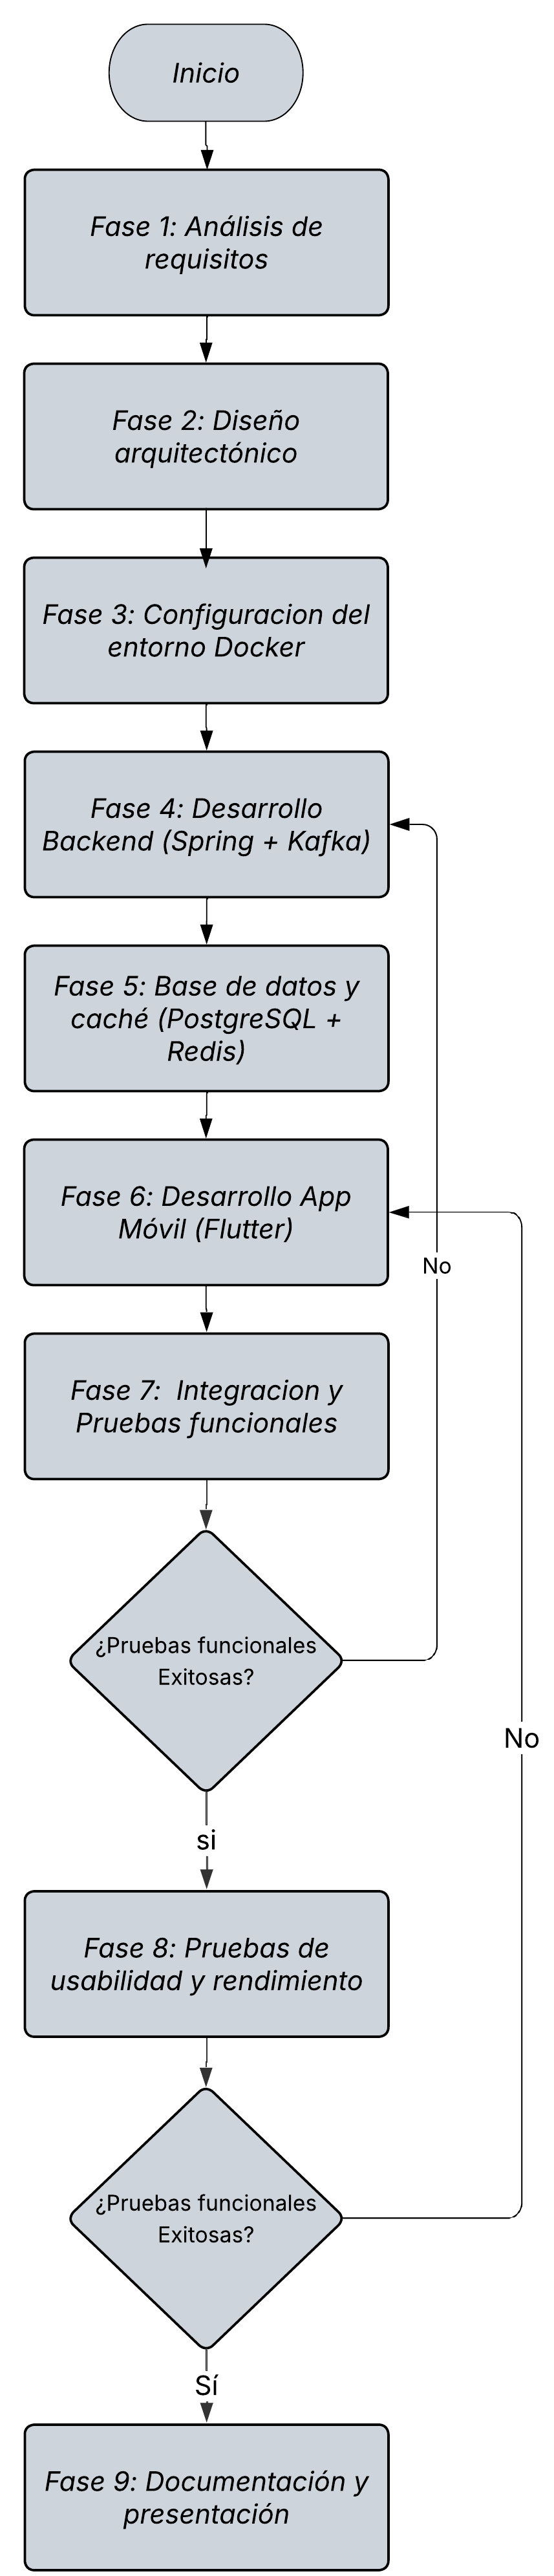
\includegraphics[width=0.20\textwidth]{imagenes/metodologia_flujo.png}
\caption{Flujo metodológico de las fases incrementales. Las flechas de retroalimentación indican ciclos de mejora.}
\label{fig:metodologia_flujo}
\end{figure}

\begin{figure}[H]
\centering
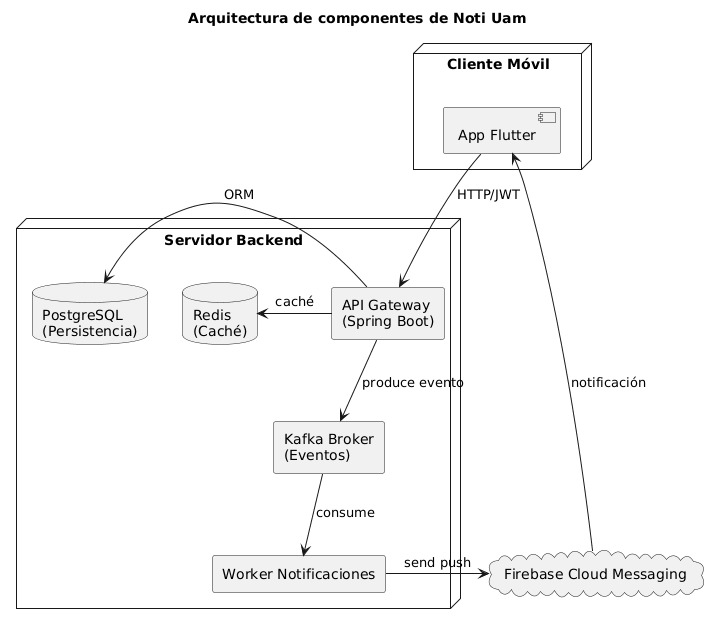
\includegraphics[width=0.30\textwidth]{imagenes/arquitectura_componentes.png}
\caption{Arquitectura de componentes de Noti Uam. El API Gateway recibe peticiones, publica eventos en Kafka; el Worker consume y envía notificaciones push.}
\label{fig:arquitectura}
\end{figure}

\begin{figure}[H]
\centering
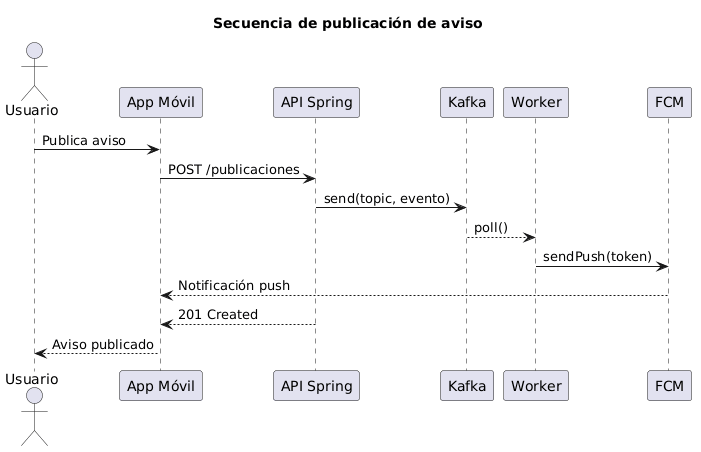
\includegraphics[width=0.30\textwidth]{imagenes/secuencia_publicacion.png}
\caption{Secuencia de publicación de un aviso y entrega de notificación push a suscriptores.}
\label{fig:secuencia}
\end{figure}

\begin{figure}[H]
\centering
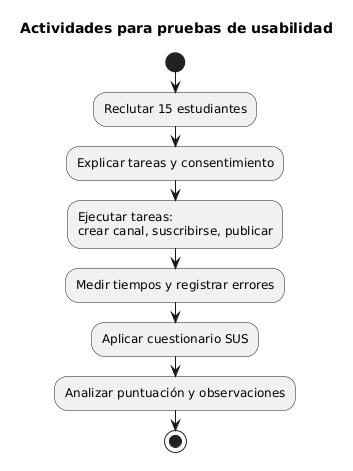
\includegraphics[width=0.35\textwidth]{imagenes/actividades_usabilidad.png}
\caption{Actividades para las pruebas de usabilidad con estudiantes.}
\label{fig:usabilidad}
\end{figure}

\subsection{Gestión de riesgos y contingencias}

La siguiente tabla identifica los principales riesgos técnicos y organizacionales, junto con sus planes de mitigación.

\begin{table}[H]
\centering
\caption{Riesgos y planes de mitigación}
\label{tab:riesgos}
\small
\begin{tabular}{|p{2cm}|p{2cm}|p{2cm}|}
\hline
\textbf{Riesgo} & \textbf{Impacto} & \textbf{Mitigación} \\
\hline
Fallo del broker Kafka & Pérdida de eventos en tiempo real & Configurar replicación de particiones y monitoreo con Prometheus; respaldo con Redis Streams como alternativa. \\
\hline
Alta latencia en notificaciones push & Mala experiencia de usuario & Optimizar la integración con FCM; usar colas de prioridad en Kafka. \\
\hline
Baja adopción en pruebas de usabilidad & Muestra insuficiente para validar hipótesis & Ofrecer incentivos; coordinar con profesores para solicitud de apoyo a la comunidad. \\
\hline
Problemas de compatibilidad entre Flutter y versiones de iOS/Android & Fallos en dispositivos reales & Probar en múltiples emuladores y dispositivos prestados; usar pruebas en la nube (Firebase Test Lab). \\
\hline
Sobrecarga de trabajo en el trimestre & Retraso en entregas & Priorizar funcionalidades críticas (MVP); aplicar metodología incremental para entregar al menos un prototipo funcional. \\
\hline
\end{tabular}
\end{table}

\subsection{Herramientas de desarrollo y colaboración}

\begin{itemize}
    \item \textbf{Control de versiones}: Git + GitHub (repositorio privado).
    \item \textbf{Gestión de tareas}: GitHub Projects o Trello, con etiquetas por fase.
    \item \textbf{CI/CD}: GitHub Actions para ejecutar pruebas unitarias automáticamente en cada \textit{push}.
    \item \textbf{Comunicación}: Discord / Slack para comunicación con el asesor.
    \item \textbf{Documentación}: Overleaf (LaTeX) para el informe y manuales.
    \item \textbf{Diagramas}: PlantUML (online) exportado a PNG.
\end{itemize}

\subsection{Criterios de aceptación final del proyecto}

Para dar por concluido el proyecto terminal, el sistema deberá cumplir con la siguiente lista de verificación:

\begin{enumerate}
    \item Todos los objetivos específicos se han alcanzado según lo documentado en las fases.
    \item La hipótesis general ha sido validada (o refutada, pero con conclusiones claras).
    \item El código fuente está disponible en un repositorio Git con un README que explique cómo ejecutar el sistema.
    \item El sistema se puede desplegar con \texttt{docker-compose up} en una máquina limpia.
    \item La puntuación SUS media es superior a 70.
    \item La documentación final (Protocolos I, II, III) ha sido aprobada por el asesor y otras autoridades pertinentes.
\end{enumerate}

La metodología descrita garantiza un desarrollo sistemático, trazable y orientado a la validación de la hipótesis, lo que es esencial para el éxito del proyecto terminal.
\section{Cronograma tentativo}

El proyecto se desarrolla en tres trimestres (Proyecto Terminal I, II y III), cada uno de 11 semanas. El diagrama siguiente muestra la distribución de actividades técnicas (basadas en las fases de la metodología) y los hitos establecidos por la CLTSI, adaptado al ancho de columna.

\begin{figure}[htbp]
\centering
\resizebox{\columnwidth}{!}{%
\begin{ganttchart}[
  hgrid,
  vgrid={*6{dotted}, *1{black}},
  x unit=0.22cm,          % muy compacto para que quepan 33 semanas
  y unit chart=0.35cm,
  title label font=\tiny\bfseries,
  bar label font=\tiny,
  bar height=0.4,
  group label font=\tiny\bfseries,
  milestone label font=\scriptsize,
  bar/.append style={fill=blue!60},
  group/.append style={fill=green!40},
  milestone/.append style={fill=red!70, rounded corners=2pt},
  link/.style={thin, -stealth}
]{1}{33}

% Títulos de los trimestres (cada 11 semanas)
\gantttitle{PT I (sem 1-11)}{11}
\gantttitle{PT II (sem 12-22)}{11}
\gantttitle{PT III (sem 23-33)}{11} \\
% Números de semana del 1 al 33
\gantttitlelist{1,...,11}{1}
\gantttitlelist{12,...,22}{1}
\gantttitlelist{23,...,33}{1} \\

% ========== ACTIVIDADES TÉCNICAS (Metodología) ==========
\ganttbar{1. Análisis de requisitos}{1}{3} \\
\ganttbar{2. Diseño arquitectónico y BD}{3}{5} \\
\ganttbar{3. Configuración entorno Docker}{6}{7} \\
\ganttbar{4. Desarrollo backend (Spring + Kafka)}{8}{16} \\
\ganttbar{5. BD y caché (PostgreSQL + Redis)}{14}{16} \\
\ganttbar{6. Desarrollo app móvil (Flutter)}{17}{22} \\
\ganttbar{7. Integración y pruebas funcionales}{23}{25} \\
\ganttbar{8. Pruebas de usabilidad y rendimiento}{26}{28} \\
\ganttbar{9. Documentación y presentación final}{29}{33} \\

% ========== HITOS CLTSI ==========
% PT I
\ganttmilestone{Envío título y asesores (sem 4)}{4} \\
\ganttmilestone{Protocolo listo (sem 7)}{7} \\
\ganttmilestone{Envío protocolo (sem 8)}{8} \\
\ganttmilestone{Envío cartel y doc final PT I (sem 11)}{11} \\
\ganttmilestone{Exposición carteles PT I (sem 12)}{12} \\
% PT II
\ganttmilestone{Envío título y asesores PT II (sem 15)}{15} \\
\ganttmilestone{Video demostrativo (sem 22)}{22} \\
\ganttmilestone{Evento exposición avances PT II (sem 23)}{23} \\
% PT III
\ganttmilestone{Envío título y asesores PT III (sem 26)}{26} \\
\ganttmilestone{Doc final a revisores (sem 30)}{30} \\
\ganttmilestone{Corrección comentarios (sem 31)}{31} \\
\ganttmilestone{Presentación final (sem 32)}{32} \\

\end{ganttchart}
}% fin de resizebox
\caption{Cronograma detallado por semanas (33 semanas = 3 trimestres de 11 semanas). Las barras azules son las fases de la metodología; los hitos rojos son entregas obligatorias según la CLTSI.}
\label{fig:cronograma_gantt}
\end{figure}

\subsection{Interpretación del cronograma}

La distribución de actividades es la siguiente:

\begin{itemize}
    \item \textbf{Trimestre I (semanas 1–11)}: Se cubren las fases 1 a 4 (inicio del backend). Se entrega el protocolo en la semana 8 y el cartel en la 11.
    \item \textbf{Trimestre II (semanas 12–22)}: Se completa el backend (fase 4), se implementa la base de datos y caché (fase 5), y se desarrolla la aplicación móvil (fase 6). El video demostrativo se entrega en la semana 22.
    \item \textbf{Trimestre III (semanas 23–33)}: Se realizan las pruebas de integración, usabilidad y rendimiento (fases 7 y 8), y se documenta el proyecto (fase 9). La presentación final ocurre en la semana 32.
\end{itemize}

Las fases 4 y 5 se solapan parcialmente (semanas 14–16) porque la base de datos y el backend se desarrollan en paralelo. Asimismo, la documentación (fase 9) comienza antes de que terminen las pruebas, para aprovechar el tiempo y permitir correcciones de última hora.

El cronograma es tentativo y podrá ajustarse durante el desarrollo, pero proporciona una guía clara para el cumplimiento de los hitos académicos.

% =========================================================
% BIBLIOGRAFÍA
% =========================================================

%\nocite{*}
\bibliographystyle{ACM-Reference-Format}
\bibliography{references}

\end{document}